En la figura~\ref{fig:diagrama-articulos-ano-metrica} se pueden visualizar las métricas de calidad, separadas por los últimos 3 años y mostrando el promedio en cada métrica de los artículos publicados en esos años, así como un apartado donde se calcula la sumatoria de estas métricas por cada año.

\begin{figure}[H]
    \centering
    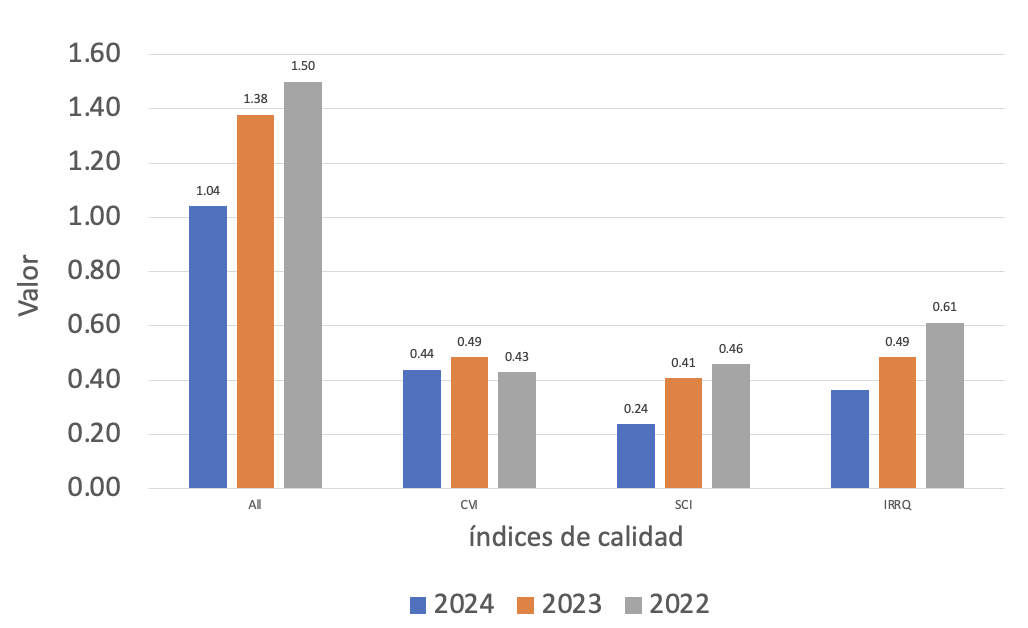
\includegraphics[scale=0.7]{tablas-images/cp2/diagrama-articulos-ano-metrica.png}
    \caption{Artículos por métricas y año}\label{fig:diagrama-articulos-ano-metrica}
\end{figure}

En la figura~\ref{fig:tipos-articulos} se muestra el conteo de artículos por su tipo específico, el cual puede ser uno de 3 opciones: 'Revista', 'Conferencia' o 'Genérico'. Vemos que la mayoría de artículos provienen de revistas.
\begin{figure}[H]
    \centering
    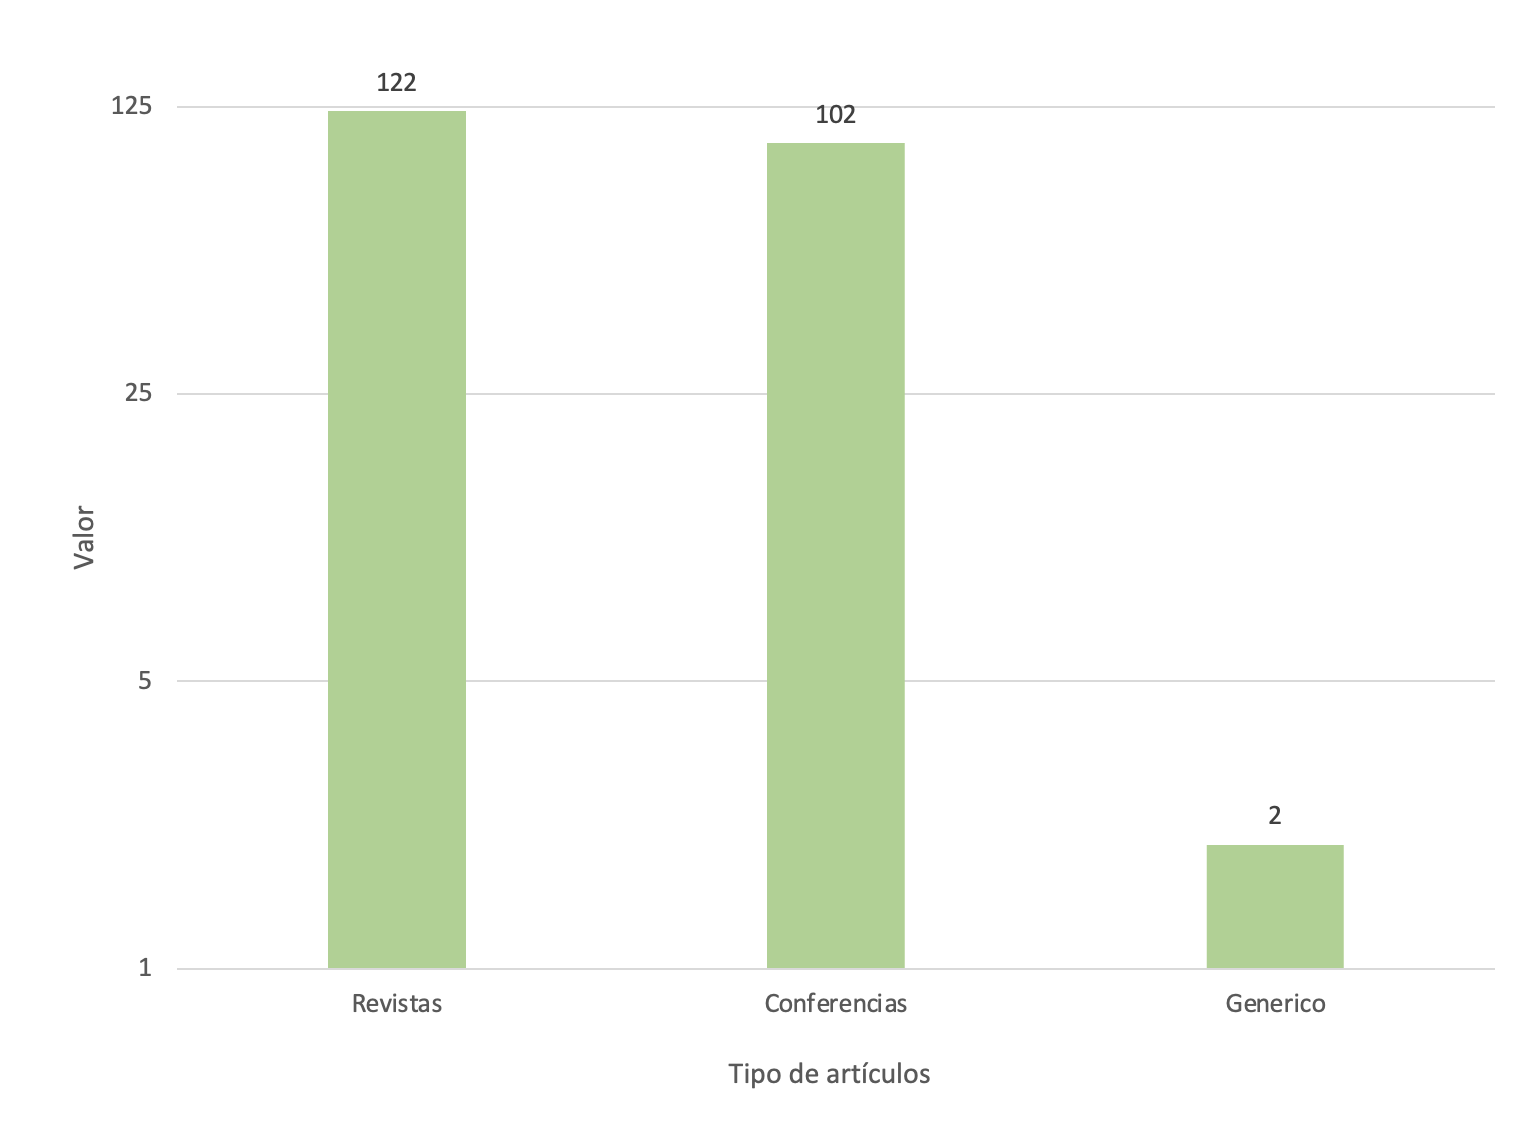
\includegraphics[scale=0.5]{tablas-images/cp2/tipos-articulos.png}
    \caption{Artículos por tipo}\label{fig:tipos-articulos}
\end{figure}

En la figura~\ref{fig:estrategia-busqueda-articulos} se detalla la cantidad de artículos que se extrajeron de cada estrategia. Se puede observar que la estrategia que generó más artículos fue la técnica de ~\textit{Snowball}.
\begin{figure}[H]
    \centering
    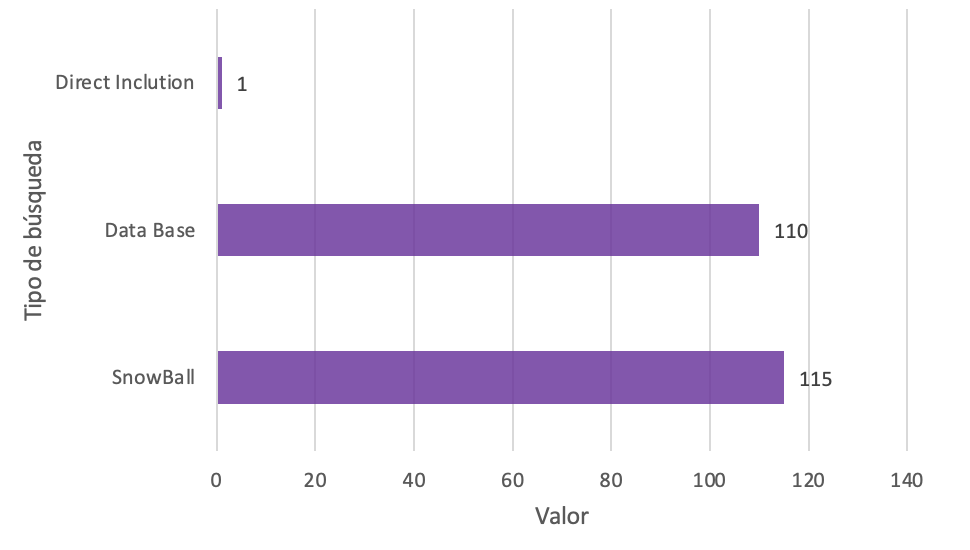
\includegraphics[scale=0.8]{tablas-images/cp2/estrategia-busqueda-articulos.png}
    \caption{Estrategia de búsqueda de artículos}\label{fig:estrategia-busqueda-articulos}
\end{figure}

Finalmente, en la figura~\ref{fig:diagrama-red-articulos} se puede apreciar un diagrama de red, que segrega por colores los tópicos más relacionados entre sí, vemos 4 grandes grupos: IA, cloud computing, virtualización, desarrollo de software.
\begin{figure}[H]
    \centering
    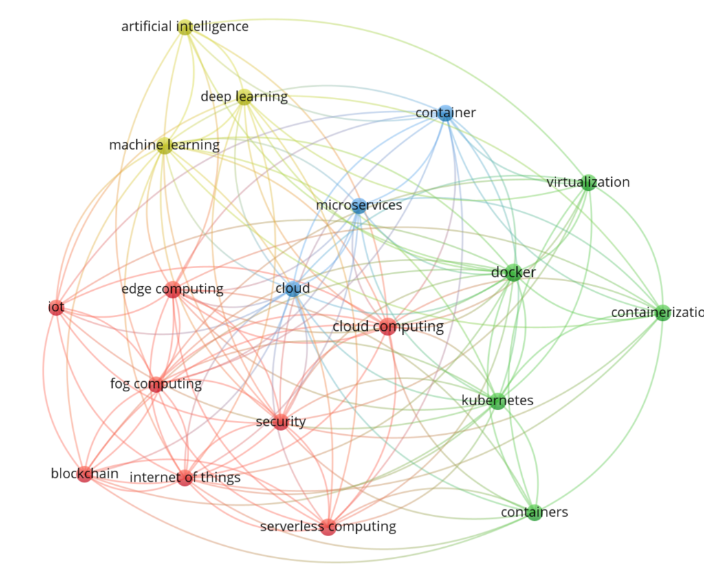
\includegraphics[scale=0.9]{tablas-images/cp2/diagrama-red-busqueda.png}
    \caption{Diagrama de red de los artículos}\label{fig:diagrama-red-articulos}
\end{figure}